% !TEX root = PREN2_Dokumentation.tex
\section{Ideen und Konzepte}
\subsection{Systemarchitektur}
Als Systemarchitektur stand die Erweiterbarkeit im Vordergrund. Allerdings sollte die Applikation durch die verwendete Architektur nicht unnötig komplex werden. Aus diesem Grund wurde bewusst gegen eine Microservicearchitektur entschieden. Die Umsetzung der Applikation mit Microservices würde zwar zu einer besseren Verteilbarkeit und Skalierung führen, der Aufwand der Umsetzung würde jedoch erheblich steigen. \\
Aus diesem Grund wurde auf eine Schichtenarchitektur gesetzt. Die klassische logische drei Schichten Architektur wurde dabei noch weiter verfeinert. Final wurde eine 6-Schichten-Architektur entworfen. Die Architektur wird zusätzlich in 3 physische Tier aufgeteilt. 

\begin{figure}[H]
	\centering
	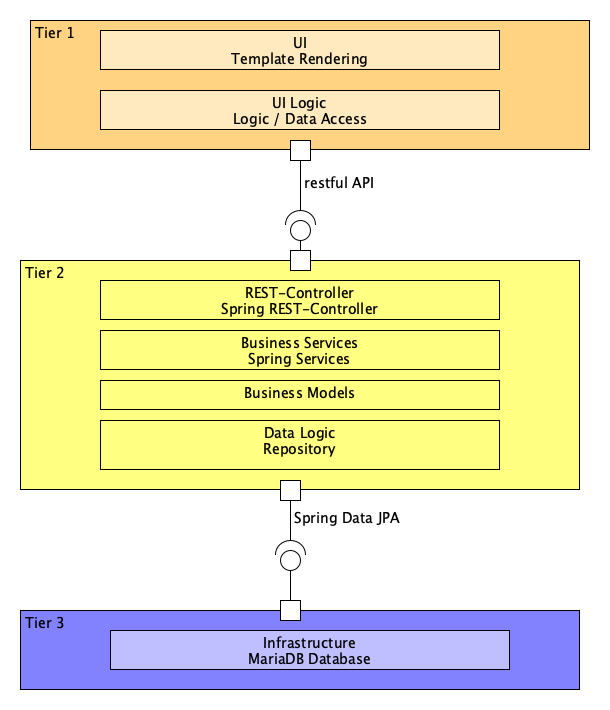
\includegraphics[width=1\textwidth]{images/architecture.png}
	\caption[Architektur]{Architektur,\\ Quelle: Autor}
	\label{img: Architektur}
\end{figure}

Die Architektur ermöglicht dabei eine sehr gute Erweiterbarkeit. Zudem kann die Software verteilt werden und unabhängig voneinander Skalieren. Durch die Aufteilung in 6 Tier wird zudem vermieden, dass die einzelnen Tiers zu breit werden. Durch das Verwenden von Frameworks kann zudem die Komplexität gering gehalten werden. Die Schnittstellen innerhalb der einzelnen Layer sind klar vorgegeben. Durch die Kommunikation via REST, bzw. die Spring Data JPA sind die Komponenten untereinander austauschbar. Die Kopplung ist sehr gering. 

\subsection{Frameworks}
\subsubsection{Spring Boot}
Spring Boot baut auf dem Spring Framework auf. Dieses bietet sich an, um performante Enterprise-Applikationen mit Java zu erstellen. Spring Boot kann dabei sehr einfach erweitert werden, sodass Spring Security, Spring Web oder Spring Data eingesetzt werden kann.\\
Spring Boot kommt dabei mit einem Tomcat Server. Dies verringert den Konfigurationsaufwand. Es ist kein Einpacken in ein .war nötig und kein zusätzliches Deployen. Zudem wird das Debugging erheblich erleichtert.  \\
Es übernimmt dabei einen grossen Teil der Beans-Konfiguration von Spring [\cite{springBoot}].\\\\
Spring Boot bietet dabei den grossen Vorteil, dass bereits Erfahrung in der Anwendung vorhanden ist. Es ist somit keine Einarbeitungszeit nötig, gängige Fehler können vermieden werden. Aus diesem Grund fiel die Entscheidung gegen Frameworks wie NodeJS. 

\subsubsection{Angular}
Angular ist ein Application Design Framework, um effiziente Single Page Applikationen zu erstellen. Es basiert auf TypeScript [\cite{angular}]. Zudem bietet Angular die Möglichkeit, als \ac{PWA} genutzt zu werden [\cite{angularPWA}]. 
Angular wurde dabei von Google entwickelt und bietet mit dem Material UI bereits viele Elemente, welche von nativen Android-Apps bekannt sind [\cite{angularMaterialUI}]. \\\\
Wie auch bei Spring ist auch bei Angular bereits Projekterfahrung vorhanden. Ein Einarbeiten ist nicht mehr nötig, die gängigsten Funktionen sind bereits bekannt. \\\\
In vorhergehenden Projekten wurde das Frontend mit unterschiedlichen Technologien umgesetzt. Einerseits kam hier Plain JavaScript zum Einsatz, andererseits wurden auch Technologien wie \gls{React} genutzt. Allerdings überzeugte Angular von all diesen am Meisten. Besonders durch die Verwendung von TypeScript wird dieses Framework hier genutzt. 

\subsection{weitere Technologien}
\subsubsection{Docker}
Docker ist eine Containertechnologie. Sie erlaubt die Erstellung und den Betrieb von Linux-Containern. Die Container sind dabei sehr leichtgewichtig und modular.\\
Die einzelnen Teile der Applikation werden in verschiedenen Containern betrieben [\cite{docker}].\\
Die Anwendung und Funktion von Docker wird in diversen Modulen an der Hochschule Luzern gelehrt. In vorhergegangenen Projekten wurde Docker bereits im selben Kontext wie hier genutzt. 

\subsubsection{MariaDB}
MariaDB ist ein OpenSource Datenbankmanagementsystem. Es ist durch die Abspaltung von MySQL entstanden. Es handelt sich dabei um ein Relationale Datenbanksystem. 
Aus Lizenzgründen wird in diesem Projekt MariaDB und nicht MySQL genutzt. Alternativ wäre auch ein Einsatz von PostgreSQL möglich. Der Unterschied zwischen PostgreSQL und MariaDB ist dabei nur marginal. Bei dieser Applikation wurde lediglich aus Erfahrung auf MariaDB gesetzt [\cite{mariadbVsPostgresql}]. \\
Durch die Verwendung von Spring Data wäre es möglich, die Datenbank im Verlauf des Projektes zu wechseln. 
\newpage